\paragraph{Введение} содержит обзор истории создания широкополосных систем и краткого рассмотрения текущих исследований в данной области.

Во введении обоснована актуальность данного исследования, проведен обзор литературы по теме диссертации, а так же
определены положения выносимые на защиту.

В диссертации рассматривается сигнал с расширенным спектром полученный методом "прямой последовательности".
Данный метод заключается в том, что гармоническая несущая сигнала модулируется высокоскоростным (широкополосным)
расширяющим сигналом. В данной работе в качестве ПСП используется код Голда. Задачи, решаемые в работе призваны
улучшить характеристики приемовычислителей Navstar GPS. Структурная схема СНС Navstar GPS представлена на рисунке
\ref{pic:sec1_gnss_system}.

\begin{figure}[H]
	\center\scalebox{1}{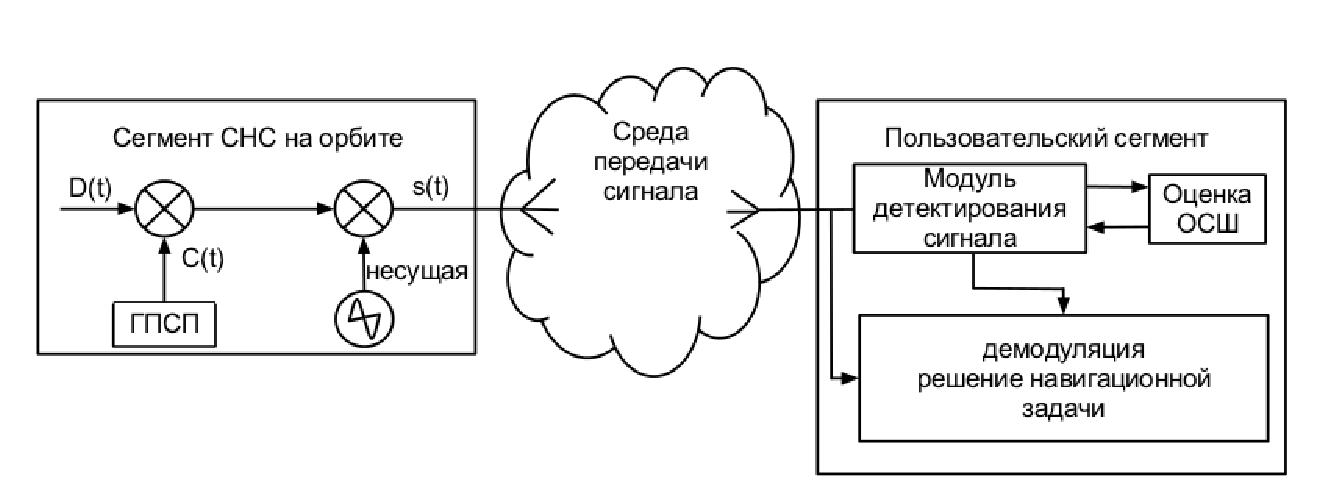
\includegraphics[width=1\linewidth]{sec1gnss_system.eps}}
	\caption{Структутраная схема СНС GPS}
	\label{pic:sec1_gnss_system}
\end{figure}

В данном типе модуляции информационные сообщения кодируются изменением фазы несущей сигнала.
Математическую модель сигнала с расширенным спектром, к которой относится система спутниковой навигации (СНС) Navstar GPS, можно представить формулой:
\begin{equation}
	\label{eq:cdma_eq}
	s_k(t)=D_k(t)C_k(t)\cos{(\omega_{k}t + \phi_k(t))} + n(t)
\end{equation}
где ${D_k}(t)$- информационный бит, ${C_k}(t)$ - расширяющий код, ${\phi_k(t)}$ - фаза обусловленная допплеровским смещением частоты, 
${n_k(t)}$ - шумовая компонента. Формула  \ref{eq:cdma_eq} представляет математическую модель сигнала для спутника номер ${k}$.
Всего в группировке спутников Navstar GPS доступно 32 спутника. После повторного модулирования сигнала, указанного в выражении \ref{eq:cdma_eq},
получается:
\begin{equation}
	\label{eq:cdma_strip_eq}
	x_k(m)=\cos{(\tilde{\omega}_{k}m + \phi_k(m))} + n_k(m) + i(m)
\end{equation}
где ${m}$ - индекс соответствующий времени, ${\tilde{\omega}_k}$ - нормированная частота, соответствующая ${\omega_k}$, ${n_k}(m)$ - шум ${n(t)}$, умноженный на ПСП,
${i(m)}$ - окрашенный шум. Окрашенный шум появляется в случае наличия других источников сигнала.
В данной работе рассматривается 2 модели сигнала: модель сигнала, соответствующая выражению \ref{eq:cdma_strip_eq}, и модель сигнала,
соответствующая выражению \ref{eq:cdma_strip_eq}, при отсутствии интерференции (${i(m)=0}$).
Информационный бит принят за константу, так как в случае смены бита гармонический характер сигнала нарушается и детектирование становится невозможным.
Так же следует учесть, что можно использовать стандартные методы нахождения битового перехода.

Интерференционная составляющая ${i(m)}$ представляет собой сигнал от других источников умноженный на ПСП искомого источника сигнала:
\begin{equation}
	\label{eq:cdma_interference}
	i(m) = C_k(t) \sum\limits_{i=1, i \ne k}^{N}C_i(t)\cos{(\omega_{i}m + \phi_i(m))}
\end{equation}

Особенность ШПС в том, что после повторной модуляции ПСП в сигнале остается только одна гармоническая компонента.
Спектр ШПС до и после снятия ПСП представлен на рисунке \ref{pic:gps_spectrum}.

\begin{figure}[H]
	\center\scalebox{1}{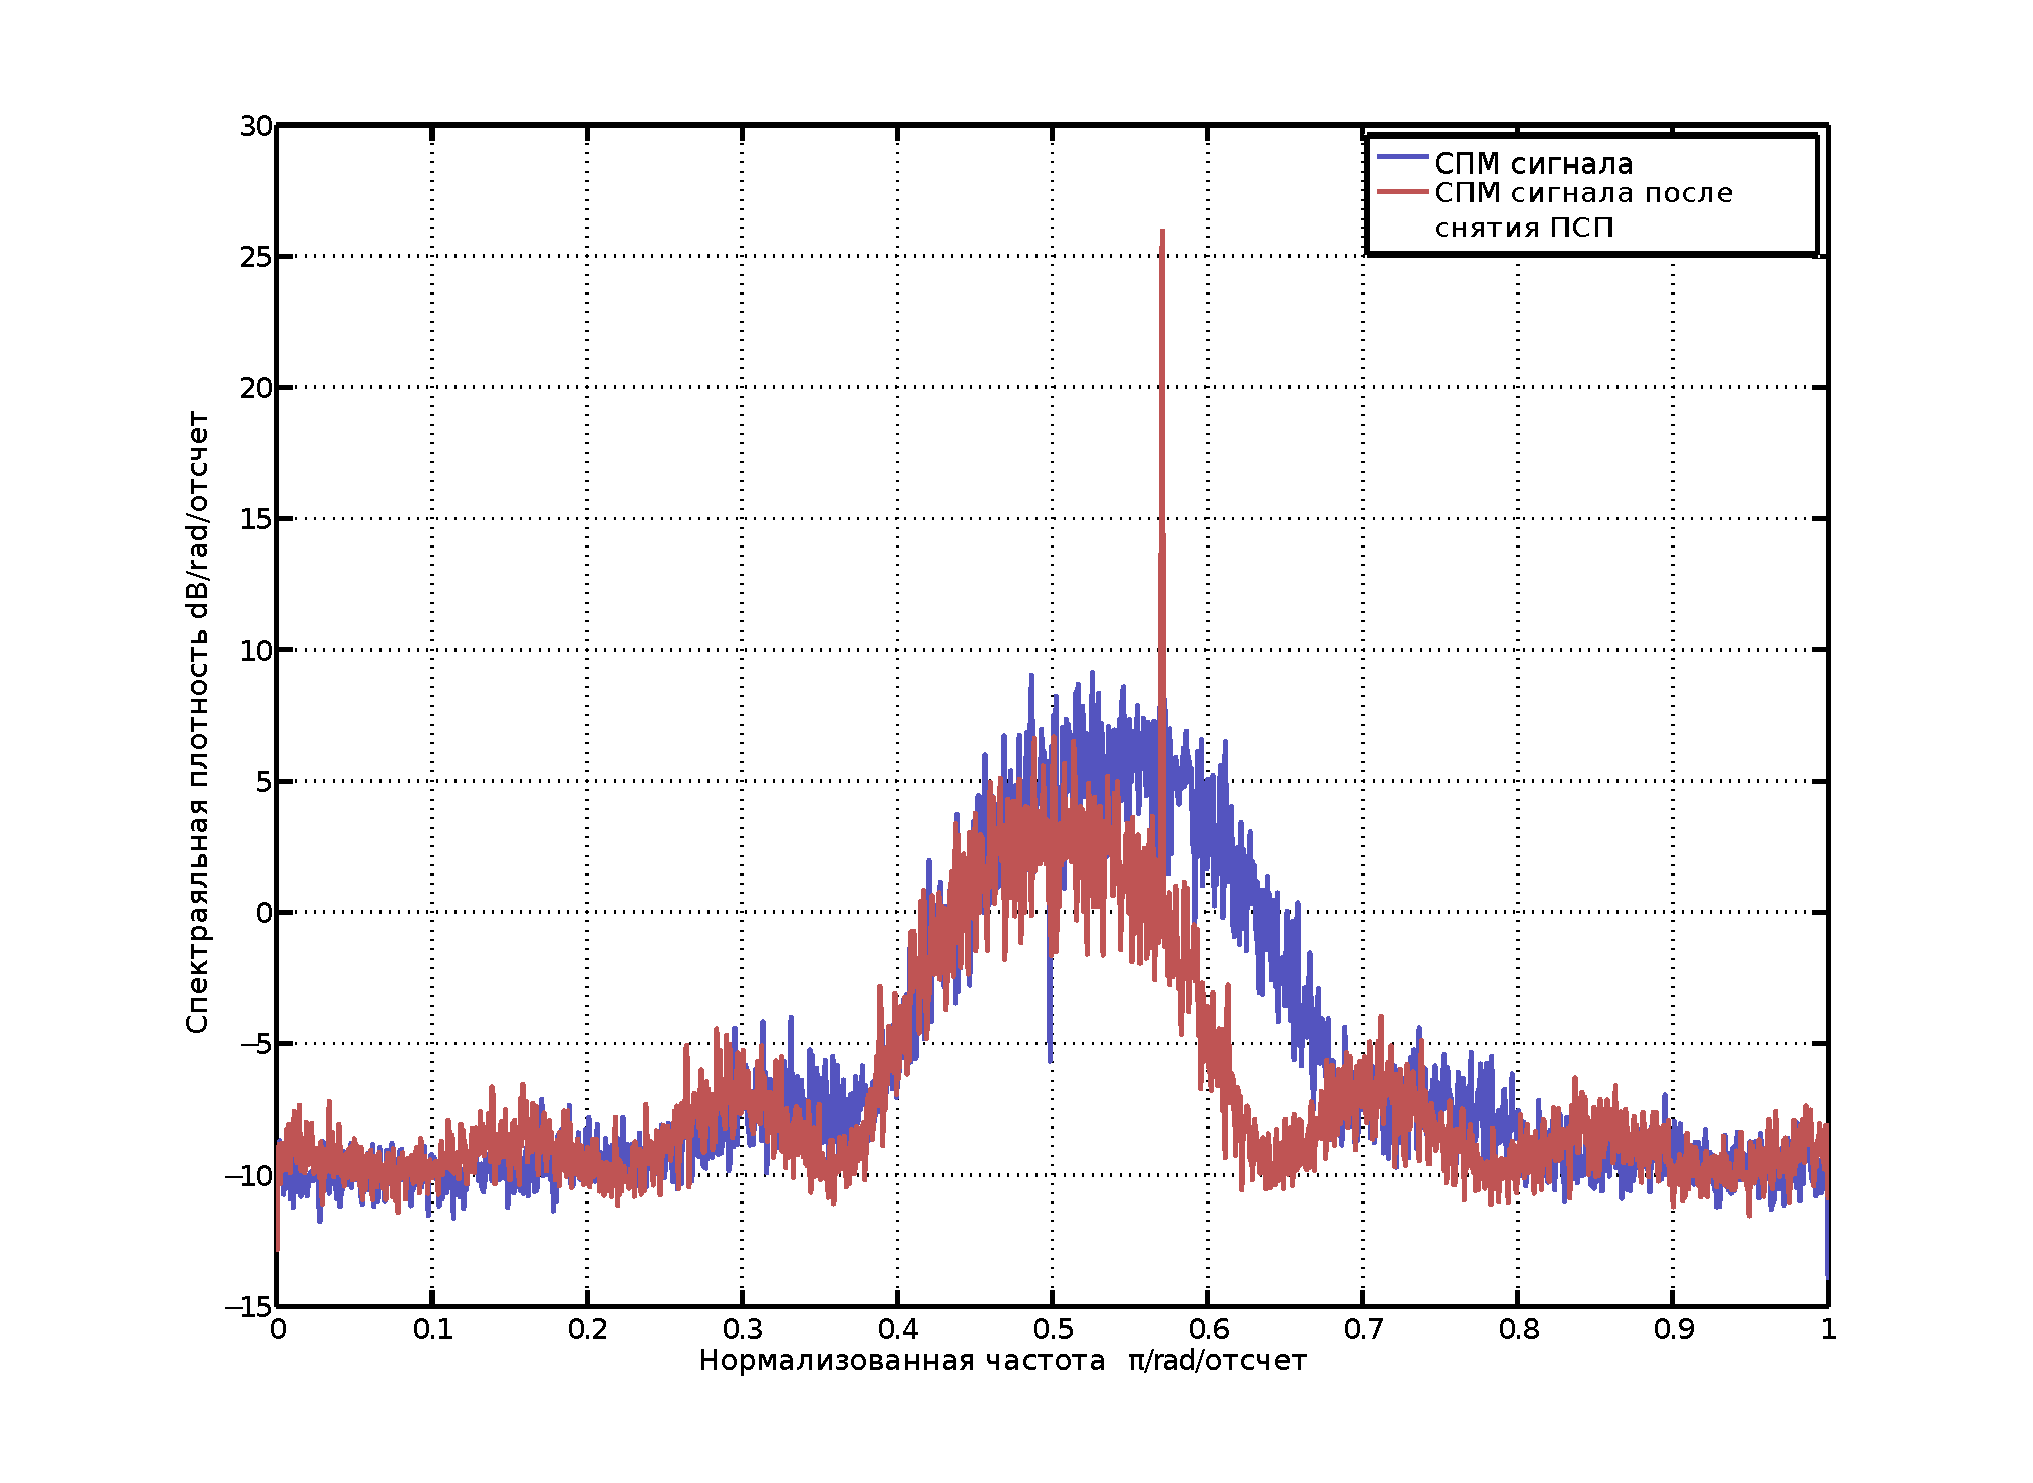
\includegraphics[width=1\linewidth]{GPS_spectra.eps}}
	\caption{Спектр ШПС сигнала}
	\label{pic:gps_spectrum}
\end{figure}
